\chapter{关于......的研究设计}
\section{变量选取}
\subsection{被解释变量}
%引用及公式撰写介绍:交叉引用公式、图表使用ref,公式在align环境中,文献引用用cite
指数由\ref{eq}表示为:
\begin{align}
taier_{it}=\sum_{j = 1}^{2}\frac{I_{i,j,t}}{I_{i,t}}\ln\left[\left(\frac{I_{i,j,t}}{I_{i,t}}\right)/\left(\frac{P_{i,j,t}}{P_{i,t}}\right)\right]\label{eq}
\end{align}



\subsection{核心解释变量}

\subsection{控制变量}
%实证中表格较长时,使用longtable环境,其余使用table环境

\begin{table}[htbp]
\zihao{5}
\centering
\caption{表格名称}
\label{tab:}
\begin{tabular}{>{\centering\arraybackslash}m{2.5cm}>{\centering\arraybackslash}m{3cm}>{\centering\arraybackslash}m{3cm}>{\centering\arraybackslash}m{5.5cm}}
\toprule
\textbf{类型} & \textbf{名称} & \textbf{符号} & \textbf{解释说明} \\
\midrule
被解释变量 & ...... & ...... & 式1\\
核心解释变量 & ......& ...... & ......\\
\multirow{2}{*}{控制变量} 
& ...... & ...... & ......\\
& ...... & ...... & ......\\

\bottomrule
\end{tabular}
\end{table}


\section{数据来源及描述性统计分析}
\subsection{主要变量}
本文数据来源于《中国统计年鉴》(2015-2024),......主要变量的描述性统计见表\ref{tab:desc_stat}。

{
\zihao{5}
\begin{longtable}{cccccc}
\caption{主要变量的描述性统计}
\label{tab:desc_stat}\\
\toprule
\textbf{变量名} & \textbf{Mean} & \textbf{Std. dev.} & \textbf{Min} & \textbf{Max} & \textbf{Observations}\\
\midrule
\endfirsthead
\multicolumn{6}{c}%
{续\tablename\thetable} \\
\toprule
\textbf{变量名} & \textbf{Mean} & \textbf{Std. dev.} & \textbf{Min} & \textbf{Max} & \textbf{Observations}\\
\midrule
\endhead
... & ... & ... & ... & ... & ... \\
\bottomrule
\end{longtable}
}


\subsection{现状分析}
图\ref{fig:province_diff_chart}展示了......情况。。
\begin{figure}[ht]
    \centering
    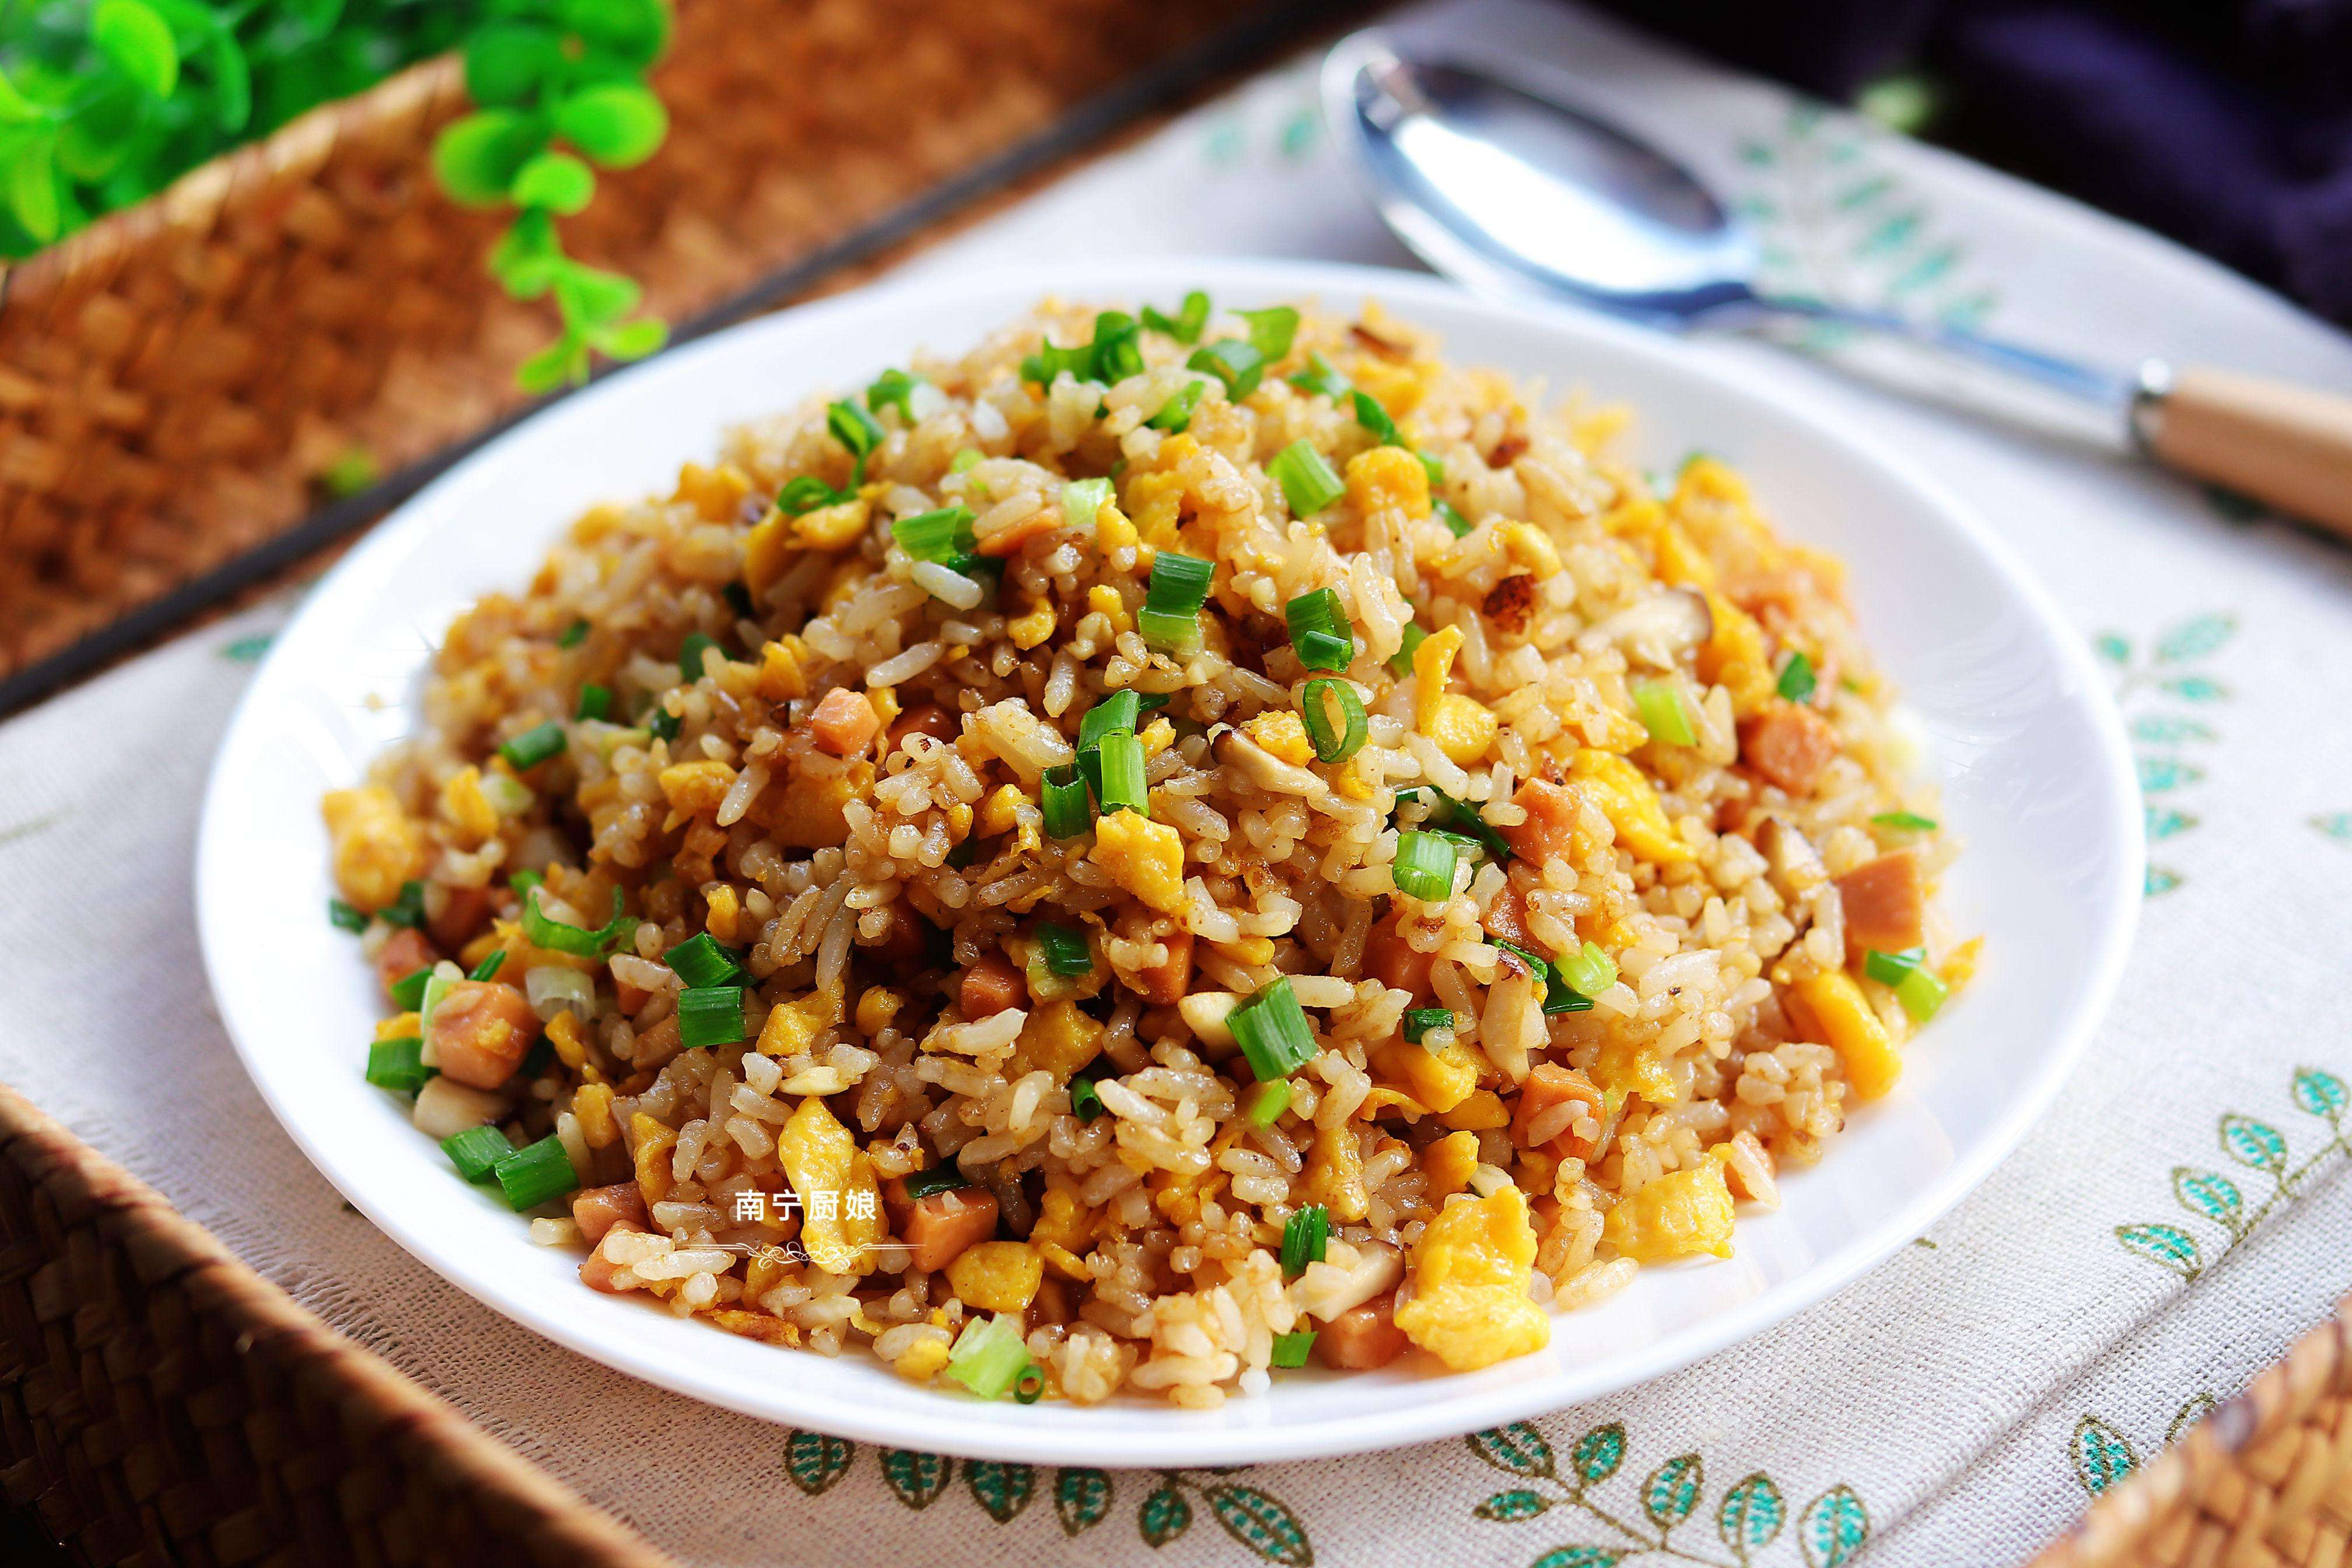
\includegraphics[scale=0.05]
    {imgs/蛋炒饭.jpeg}
    \caption{图名}
    \label{fig:province_diff_chart}
\end{figure}


\section{模型设定}
本文数据为.......模型:







